\chapter{Soccer Simulation League 3D}
\label{Soccer Simulation League 3D}

\section{SimSpark}
SimSpark is a generic physical multiagent simulator system for agents in three-dimensional environments. It builds on the flexible Spark application framework.
It is used as the official Robocup 3D simulation server. In comparison to specialized simulators, users can create new simulations by using a scene description language. SimSpark is a powerful tool to state different multi-agent research questions.
\section{Soccer simulation}
RoboCup is an initiative to foster artificial intelligence and robotics research by providing a standard problem in the form of robot soccer competitions. { \bf rcssserver3d} is the official competition environment for the 3D Soccer Simulation League at RoboCup. It implements a soccer simulation where two teams of up to eleven humanoid robots play against each other. You can see the soccer field in figure \ref{fig:SimulationSoccerField}.
\begin{figure}[ht!]
\centering
  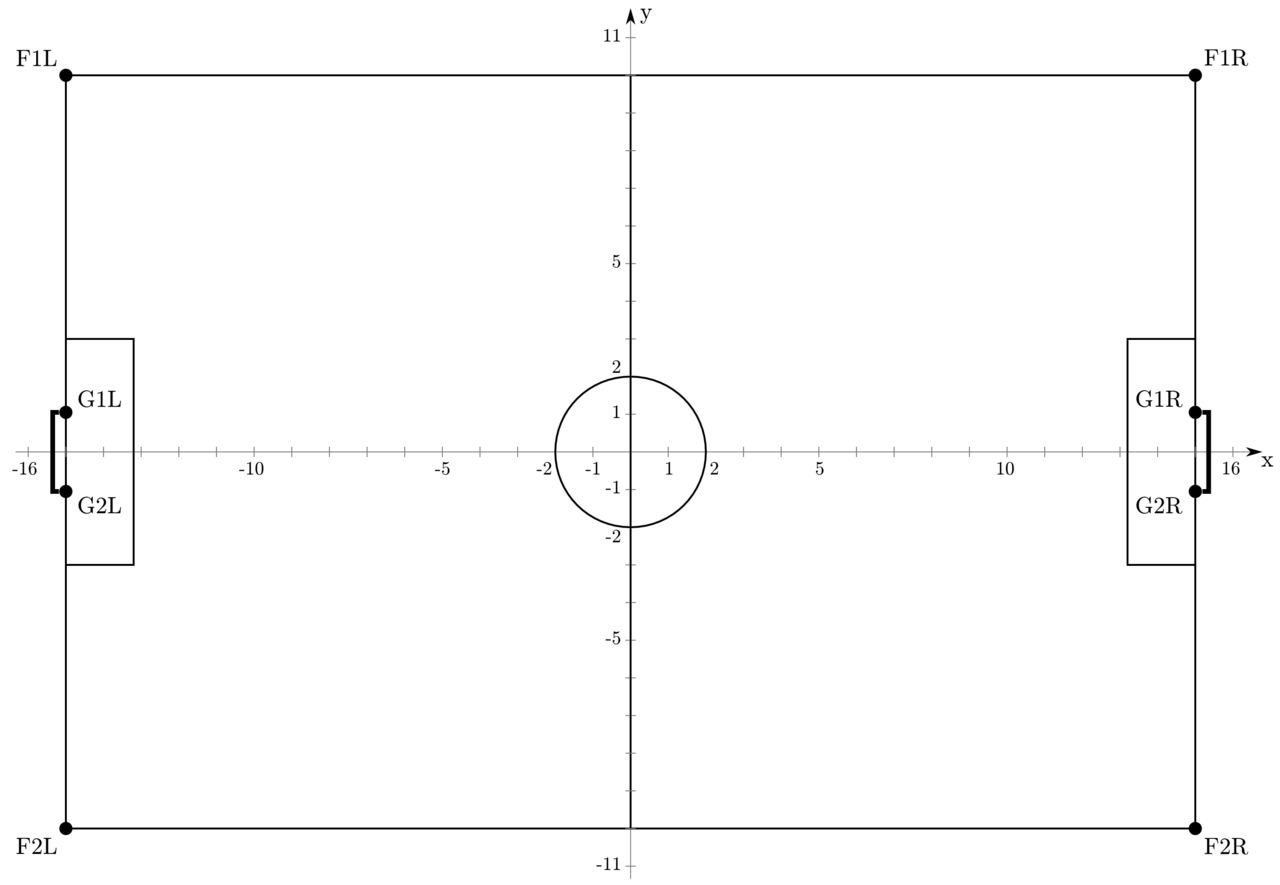
\includegraphics[scale=1.2]{Chapter2/figures/1280px-SoccerSimulation_FieldPlan.png}
  \caption{Simulation Soccer Field} 
  \label{fig:SimulationSoccerField}
\end{figure}
\section{Server}
The SimSpark server hosts the simulation process that manages the simulation. It is responsible for advancing the simulation. The simulation state is constantly modified during the Simulation Update Loop.
Objects in the scene change their state, i.e. one ore more of their properties like position, speed or angular velocity changes due to several influences. They are under the control of a rigid body physical simulation, that resolves collisions, applies drag, gravity etc. Agents that take part in the simulation also modify objects with the help of their effectors.
Another responsibility of the server is to keep track of connected agent processes. Each simulation cycle the server collects and reports sensor information for each of the sensors of all connected agents. It further carries out received action sequences that an agent triggers using its available effectors.
The server can, depending upon its config, renders the simulation itself. It implements an internal monitor that omits the network overhead. Additionally, it supports streaming data to remote monitor processes which take responsibility for rendering the 3D scene.
\section{Simulation Update Loop}
SimSpark implements a simple internal event model that immediately executes every action received from an agent. It does not try to compensate any network latency or compensate for different computing resources available to the connected agents.A consequence is that SimSpark currently does not guarantee that events are reproducible. This means repeated simulations may have a different outcome, depending on network delays or load variations on the machines hosting the agents and the server.
\section{Network Protocol}
The server exposes a network interface to all agents, on TCP port 3100 by default.
When an agent connects to the server the agent must first send a CreateEffector message followed by a InitEffector message.
Once established, the server sends groups of messages to the agent that contain the output of the agent's perceptors, including any hinge positions of the model, any heard messages, seen objects, etc. The exact messages sent depend upon the model created for the agent. Details of effector messages are given on the perceptors page. In response to these perceptor messages, the agent may influence the simulation by sending effector messages. These perform tasks such as moving hinges in the model. Details of effector messages are given on the effectors section.
\section{Monitor}
The SimSpark monitor is responsible for rendering the current simulation. It connects to a running server instance from which it continuously receives a stream of updates that describe the simulation state either as full snapshots or as incremental updates.
The format of the data stream that the server sends to the monitor is called Monitor Format. It is a customizable language used to describe the simulation state.
Apart from describing the pure simulation state each monitor format may provide a mechanism to transfer additional game specific state. For the soccer simulation this means for example current play mode and goals scored so far.The monitor client itself only renders the pure scene and defers the rendering of the game state to plugins. These plugins are intended to parse the game state and display it as an overlay, e.g. print out playmode and scores on screen.
\section{Perceptors}
Perceptors are the senses of an agent, allowing awareness of the agent's model state and the environment.
The server sends perceptor messages to agents, via the network protocol, for every cycle of the simulation.
Perceptor messages are sent via the network protocol.There are both general perceptors that apply to all simulations, and soccer perceptors that are specific to the soccer simulation.



\subsection{General perceptors}

\begin{description}



  \item [GyroRate Perceptor]
  The gyro rate perceptor delivers information about the change in orientation of a body. The message contains the GYR identifier, the name of the body to which the gyro perceptor belongs and three rotation angles. These rotation angles describe the change rates in orientation of the body during the last cycle. In other words the current angular velocities along the three axes of freedom of the corresponding body in degrees per second. To keep track of the orientation of the body, the information to each gyro rate perceptor is sent every cycle.
  \begin{description}
  \item[{\bf Message format:}]
  \begin{verbatim}
  (GYR (n <name>) (rt <x> <y> <z>))
  \end{verbatim}
  \item[{\bf Frequency:}]
  Every cycle
  \end{description}




  \item [HingeJoint Perceptor]
  A hinge joint perceptor receives information about the angle of the correponding single-axis hinge joint. It contains the identifier HJ, the name of the perceptor and the position angle of the axis in degrees. A zero angle corresponds to straightly aligned bodies. The position angle of each hinge joint perceptor is sent every cycle.
Each hinge joint has minimum and maximum limits on its angular position. This varies from hinge to hinge and depends upon the model being used.  \begin{description}
  \item[{\bf Message format:}]
  \begin{verbatim}
  (HJ (n <name>) (ax <ax>))
  \end{verbatim}
  \item[{\bf Frequency:}]
  Every cycle
  \end{description}
  
  
  
  \item [ForceResistance Perceptor]
  This perceptor informs about the force that acts on a body. After the identifier FRP and the name of the body the perceptor message contains two vectors. The first vector describes the point of origin relative to the body itself and the second vector the resulting force on this point. The two vectors are just an approximation about the real applied force. The point of origin is calculated as weighted average of all contact points to which the force is applied, while the force vector represents the total force applied to all of these contact points. The information to a force resistance perceptor is just sent in case of a present collision of the corresponding body with another simulation object. If there is no force applied, the message of this perceptor is omitted.
 \begin{description}
  \item[{\bf Message format:}]
  \begin{verbatim}(FRP (n <name>) (c <px> <py><pz>)
   (f <fx><fy><fz>))
  \end{verbatim}
  \item[{\bf Frequency:}]
  Every cycle, but only in case of a present    		collision.
  \end{description}




  \item [Accelerometer]
  This perceptor measures the proper acceleration it experiences relative to free fall. As a consequence an accelerometer at rest relative to the Earth's surface will indicate approximately 1g upwards. To obtain the acceleration due to motion with respect to the earth, this gravity offset should be subtracted.
    \begin{description}
  \item[{\bf Message format:}]
  \begin{verbatim}
  (ACC (n <name>) (a <x> <y> <z>))
  \end{verbatim}
  \item[{\bf Frequency:}]
  Every cycle
  \end{description}
\end{description}

\subsection{General perceptors}
\begin{description}
  \item [Vision Perceptor]
  The Vision perceptor delivers information about seen objects in the environment, where objects are either others players, the ball, field-lines or markers on the field. Currently there are 8 markers on the field: one at each corner point of the field and one at each goal post. With each visible object you get a vector described in spherical coordinates. In other words the distance together with the horizontal and latitudal angle to the center of a visible object relative to the orientation of the camera.
 \begin{description}
  \item[{\bf Message format:}]
  \begin{verbatim}
  (See +(<name> (pol <distance> <angle1>
   <angle2>))+(P (team <teamname>) (id <playerID>)
    + (<bodypart> (pol <distance> <angle1> <angle2
    >)))+(L (pol <distance> <angle1> <angle2>)(pol
     <distance> <angle1> <angle2>)))
  \end{verbatim}
  \item[{\bf Frequency:}]
 Every third cycle (every 0.06 seconds)
  \end{description}





  \item [GameState Perceptor]
  The game state perceptor delivers several information about the actual state of the soccer game environment. A game state message is started with the GS identifier, followed by a list of different state information. Currently just the actual play time and play mode are transmitted in each cycle. Play time starts from zero at kickoff of the first half, and 300 at kickoff of the second half and is given as a floating point number in seconds, to two decimal places.
     \begin{description}
  \item[{\bf Message format:}]
  \begin{verbatim}
  (GS (t <time>) (pm <playmode>))
  \end{verbatim}
  \item[{\bf Frequency:}]
 Every cycle
  \end{description}





  \item [Hear Perceptor]
  Agent processes are not allowed to communicate with each other directly, but agents may exchange messages via the simulation server. For this purpose agents are equipped with the so-called hear perceptor, which serves as an aural sensor and receives messages shouted by other players. 
  \begin{description}
  \item[{\bf Message format:}]
  \begin{verbatim}
  (hear <time> self/<direction> <message>)
  \end{verbatim}
  \item[{\bf Frequency:}]
  Every cycle
  \end{description}

\end{description}
\section{Effectors}
Effectors allow agents to perform actions within the simulation. Agents control them by sending messages to the server, and the server changes the game state accordingly. Effectors are the logical dual of perceptors.
Effector control messages are sent via the network protocol. Details of each message type are shown in each section below.
There are both general effectors that apply to all simulations, and soccer effectors that are specific to the soccer simulation.\\
\subsection{General Effectors}
\begin{description}
  \item [Create Effector]
  When an agent initially connects to the server it is invisible and cannot take affect a simulation in any meaningful way. It only possesses a so-called CreateEffector. An agent uses this effector to advice the server to construct it according to a scene description file it passes as a parameter. This file is used to construct the physical representation and all further effectors and perceptors.
  \begin{description}
  \item[{\bf Message format:}]
  \begin{verbatim}
  (scene <filename>)
  \end{verbatim}
  \end{description}

  \item [HingeJoint Effector]
  Effector for all axis with a single degree of freedom. The first parameter is the name of the axis. The second parameter is a speed value, passed in radians per second. Setting a speed value on a hinge means that the speed will be maintained until a new value is provided. Even if the hinge meets its extremity, it will bounce around at the extremity until a new speed value is requested.
  \begin{description}
  \item[{\bf Message format:}]
  \begin{verbatim}
  (<name> <ax>)
  \end{verbatim}
  \end{description}

  \item [Synchronize Effector]
  Agents running in Agent Sync Mode must send this command at the end of each simulation cycle. Note that the server ignores this command if it is received in Real-Time Mode, so it is safe to configure your agent to always append this command to your agent's responses.
  \begin{description}
  \item[{\bf Message format:}]
  \begin{verbatim}
  (syn)
  \end{verbatim}
  \end{description}

\end{description}

\subsection{Soccer Effectors}
\begin{description}
  \item [Init Effector]
  The init command is sent once for each agent after the create effector sent the scene command. It registers this agent as a member of the passed team with the passed number. All players of one team have to use the same teamname and different player number values.
  \begin{description}
  \item[{\bf Message format:}]
  \begin{verbatim}
  (init (unum <playernumber>)
  (teamname <yourteamname>))
  \end{verbatim}
  \end{description}



  \item [Beam Effector]
  The beam effector allows a player to position itself on the field before the start of each half. The x and y coordinates define the position on the field with respect to the field's coordinate system, where (0,0) is the absolute center of the field.
  \begin{description}
  \item[{\bf Message format:}]
  \begin{verbatim}
  (beam <x> <y> <rot>)
  \end{verbatim}
  \end{description}



  \item [Say Effector]
  The say effector permits communication among agents by broadcasting messages. In order to say something, the following command has to be employed.
  \begin{description}
  \item[{\bf Message format:}]
  \begin{verbatim}
  (say <message>)
  \end{verbatim}
  \end{description}

\end{description}
\section{Model}
SimSpark comes with Nao robot model for use by agents. The physical representation of each model is stored in an .rsg file.The Nao humanoid robot manufactured by Aldebaran Robotics. Its height is about 57cm and its weight is around 4.5kg. Its biped architecture with 22 degrees of freedom allows Nao to have great mobility. { \bf rcssserver3d} simulates Nao nicely.
\begin{figure}[ht]
\centering
  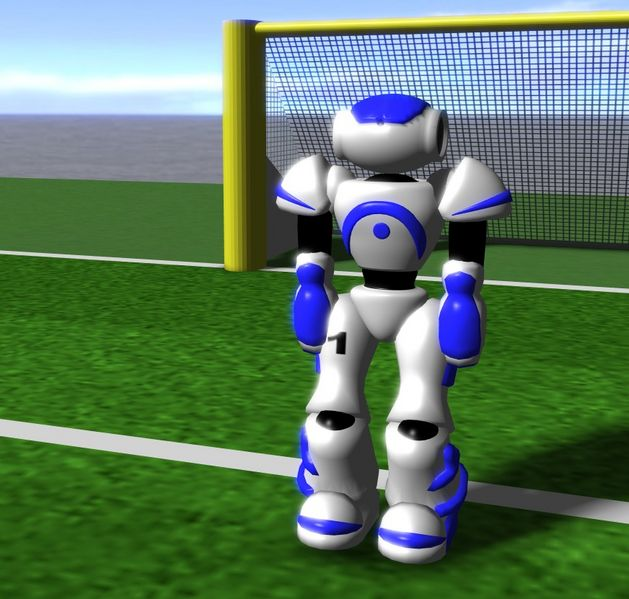
\includegraphics[scale=0.3]{Chapter2/figures/629px-Models-nao.jpg}
  \caption{Nao in simulation monitor} 
  \label{fig:Naoinsimulationscreen}
\end{figure}